\documentclass[
	10pt,								% globale Schriftgröße
	parskip=half-,						% setzt Absatzabstand hoch
	paper=a4,							% Format
	english,ngerman,					% lädt Sprachpakete
	]{scrartcl}							% Dokumentenklasse

% //////////////////// Pakete laden ////////////////////
\usepackage[fleqn]{amsmath}
\usepackage[fleqn]{mathtools}
\usepackage{amssymb}			% mathematische symbole, für \ceckmarks
\usepackage{amsthm}				% für proof
\usepackage{mathrsfs}			% für \mathscr
\usepackage{latexsym}
\usepackage{marvosym}				% für Lightning

\usepackage{fontspec} 			% funktioniert nur mit den neueren Compilern z.B. XeLaTeX
\usepackage{microtype}			% für bessere Worttrennung
\usepackage[ngerman]{babel} 	% Spracheinstellung
\usepackage{lmodern}			% verändert verwendete Schriftart, damit sie weniger pixelig ist

\usepackage{verbatim}
\usepackage{listings}			% Für Quellcode

\usepackage{graphicx}
\usepackage{tabularx}			% für Tabellen mit gleicher Spaltenbreite und automatischen Umbrüchen
\usepackage{fullpage}
\usepackage{multirow}			% für multirow in tabulars
\usepackage{rotate}
\usepackage[cmyk,table]{xcolor} % um Farben zu benutzen, kann mehr als das Paket color
\usepackage[					% Verlinkungen
	colorlinks,					% farbige Schrift, statt farbiger Rahmen
	linktocpage,				% verlinkt im Abb.Verzeichnis Seitenzahl statt Bildunterschrift
	linkcolor=blue				% setzt Farbe der Links auf blau
	]{hyperref}					% nur für digitale Anwendungen, url = "http://www.example.com"
\usepackage{url}				% für Webadressen wie e-mail usw.: "\url{http://www.example.com}"

\usepackage{enumerate}			% für versch. Aufzählungezeichen wie z.B. a)
\usepackage{xspace}				% folgt ein Leerzeichen nach einem \Befehl, wird es nicht verschluckt.
\usepackage{cancel}				% für das Durchstreichen u.a. in Matheformeln mit \cancel
\usepackage{float}              % zum Forcieren der Position von figure-Umgebungen

% zum Zeichnen (u.a. von Graphen)
\usepackage{fp}
\usepackage{tikz}
\usetikzlibrary{tikzmark}			% für \tikzmark{toRemember}
\usetikzlibrary{positioning}	% verbesserte Positionierung der Knoten
\usetikzlibrary{automata}		% für Automaten (GTI)
\usetikzlibrary{arrows}
\usetikzlibrary{shapes}
\usetikzlibrary{decorations.pathmorphing}
\usetikzlibrary{decorations.pathreplacing}
\usetikzlibrary{decorations.shapes}
\usetikzlibrary{decorations.text}

% //////////////////// Syntaxhighlighting ////////////////////
\lstloadlanguages{Python, Haskell, [LaTeX]TeX, Java}
\lstset{
   basicstyle=\footnotesize\ttfamily,	% \scriptsize the size of the fonts that are used for the code
   backgroundcolor = \color{bgcolour},	% legt Farbe der Box fest
   breakatwhitespace=false,	% sets if automatic breaks should only happen at whitespace
   breaklines=true,			% sets automatic line breaking
   captionpos=t,				% sets the caption-position to bottom, t for top
   commentstyle=\color{codeblue}\ttfamily,% comment style
   frame=single,				% adds a frame around the code
   keepspaces=true,			% keeps spaces in text, useful for keeping indentation
							% of code (possibly needs columns=flexible)
   keywordstyle=\bfseries\ttfamily\color{codepurple},% keyword style
   numbers=left,				% where to put the line-numbers;
   							% possible values are (none, left, right)
   numberstyle=\tiny\color{codegreen},	% the style that is used for the line-numbers
   numbersep=5pt,			% how far the line-numbers are from the code
   stepnumber=1,				% nummeriert nur jede i-te Zeile
   showspaces=false,			% show spaces everywhere adding particular underscores;
							% it overrides 'showstringspaces'
   showstringspaces=false,	% underline spaces within strings only
   showtabs=false,			% show tabs within strings adding particular underscores
   flexiblecolumns=false,
   tabsize=1,				% the step between two line-numbers. If 1: each line will be numbered
   stringstyle=\color{orange}\ttfamily,	% string literal style
   numberblanklines=false,				% leere Zeilen werden nicht mitnummeriert
   xleftmargin=1.2em,					% Abstand zum linken Layoutrand
   xrightmargin=0.4em,					% Abstand zum rechten Layoutrand
   aboveskip=2ex, 
}

\lstdefinestyle{py}{
   language=Python,
}
\lstdefinestyle{hs}{
   language=Haskell,
}
\lstdefinestyle{tex}{
	language=[LaTeX]TeX,
	escapeinside={\%*}{*)},     % if you want to add LaTeX within your code
	texcsstyle=*\bfseries\color{blue},% hervorhebung der tex-Schlüsselwörter
	morekeywords={*,$,\{,\},\[,\],lstinputlisting,includegraphics,
	rowcolor,columncolor,listoffigures,lstlistoflistings,
	subsection,subsubsection,textcolor,tableofcontents,colorbox,
	fcolorbox,definecolor,cellcolor,url,linktocpage,subtitle,
	subject,maketitle,usetikzlibrary,node,path,addbibresource,
	printbibliography},% if you want to add more keywords to the set
     numbers=none,
     numbersep=0pt,
     xleftmargin=0.4em,
}

\lstdefinestyle{java}{
	language=Java,
	extendedchars=true,		% lets you use non-ASCII characters;
   						% for 8-bits encodings only, does not work with UTF-8
}

\lstdefinelanguage[x64]{Assembler}     % add a "x64" dialect of Assembler
   [x86masm]{Assembler} % based on the "x86masm" dialect
   % with these extra keywords:
   {morekeywords={CDQE,CQO,CMPSQ,CMPXCHG16B,JRCXZ,LODSQ,MOVSXD, %
                  POPFQ,PUSHFQ,SCASQ,STOSQ,IRETQ,RDTSCP,SWAPGS, %
                  rax,rdx,rcx,rbx,rsi,rdi,rsp,rbp, %
                  r8,r8d,r8w,r8b,r9,r9d,r9w,r9b}
}					% for 8-bits encodings only, does not work with UTF-8

\lstdefinestyle{c}{
	language=c,
	extendedchars=true,		% for 8-bits encodings only, does not work with UTF-8
}

% //////////////////// eigene Kommandos ////////////////////
\newcommand\FU{Freie Universität Berlin\xspace}% benötigt package xspace
\newcommand\gdw{g.\,d.\,w.\xspace}
\newcommand\oBdA{o.\,B.\,d.\,A.\xspace}
\newcommand{\Eu}{\texteuro}
\newcommand\N{\mathbb{N}\xspace}
\newcommand\Q{\mathbb{Q}\xspace}
\newcommand\R{\mathbb{R}\xspace}
\newcommand\Z{\mathbb{Z}\xspace}
\newcommand\ohneNull{\ensuremath{\backslash\lbrace 0\rbrace}}% \{0}
\let\dhALT\dh	% Schreibt Befehl \dh in \dhALT um
\renewcommand\dh{d.\,h.\xspace}	%renew überschreibt command \dh
\newcommand\Bolt{\;\text{\LARGE\raisebox{-0.3em}{\Lightning}\normalsize}\xspace}% Blitz
\newcommand\zz{\ensuremath{\raisebox{+0.25ex}{Z}% zu zeigen
			\kern-0.4em\raisebox{-0.25ex}{Z}%
			\;\xspace}}
\newcommand{\from}{\ensuremath{\colon}}
\newcommand{\floor}[1]{\lfloor{#1}\rfloor}
\newcommand{\ceil}[1]{\lceil{#1}\rceil}
 \renewcommand{\L}{\ensuremath{\mathcal{L}}\xspace}
 \renewcommand{\P}{\ensuremath{\mathcal{P}}\xspace}
 \newcommand{\NL}{\ensuremath{\mathcal{N}\kern-0.2em\mathcal{L}}\xspace}
 \newcommand{\NP}{\ensuremath{\mathcal{NP}}\xspace}

% //////////////////// Mathefunktionen ////////////////////
\DeclareMathOperator{\Landau}{\mathcal{O}}
\DeclareMathOperator{\True}{True}
\DeclareMathOperator{\False}{False}

% //////////////////// eigene Theoreme ////////////////////
\newtheorem{theorem}{Satz}
\newtheorem{corollary}[theorem]{Folgerung}
\newtheorem{lemma}[theorem]{Lemma}
\newtheorem{observation}[theorem]{Beobachtung}
\newtheorem{definition}[theorem]{Definition}
\newtheorem{Literatur}[theorem]{Literatur}
% konfiguriert proof
\makeatletter
\newenvironment{Proof}[1][\proofname]{\par
  \pushQED{\qed}%
  \normalfont \topsep6\p@\@plus6\p@\relax
  \trivlist
  \item[\hskip\labelsep
%         \itshape
        \bfseries
    #1\@addpunct{.}]\ignorespaces
}{%
  \popQED\endtrivlist\@endpefalse
}
\makeatother

% //////////////////// eigene Farben ////////////////////
\let\definecolor=\xdefinecolor
\definecolor{FUgreen}{RGB}{153,204,0}
\definecolor{FUblue}{RGB}{0,51,102}

\definecolor{middlegray}{rgb}{0.5,0.5,0.5}
\definecolor{lightgray}{rgb}{0.8,0.8,0.8}
\definecolor{orange}{rgb}{0.8,0.3,0.3}
\definecolor{azur}{rgb}{0,0.7,1}
\definecolor{yac}{rgb}{0.6,0.6,0.1}
\definecolor{Pink}{rgb}{1,0,0.6}

\definecolor{bgcolour}{rgb}{0.97,0.97,0.97}
\definecolor{codegreen}{rgb}{0,0.6,0}
\definecolor{codegray}{rgb}{0.35,0.35,0.35}
\definecolor{codepurple}{rgb}{0.58,0,0.82}
\definecolor{codeblue}{rgb}{0.4,0.5,1}

% //////////////////// eigene Settings ////////////////////

\textheight = 230mm		% Höhe des Satzspiegels / Layouts
\footskip = 10ex			% Abstand zw. Fußzeile und Grundlinie letzter Textzeile
\parindent 0pt			% verhindert Einrückung der 1. Zeile eines Absatzes
\setkomafont{sectioning}{\rmfamily\bfseries}% setzt Ü-Schriften in Serifen, {disposition}											% bindet Header ein (WICHTIG)
\usepackage{graphicx}
\usepackage{amsmath}
\usepackage{amssymb}
\usepackage{fancyvrb}

\newcommand{\dozent}{Prof. R. Rojas}					% <-- Names des Dozenten eintragen
\newcommand{\projectNo}{8}
\newcommand{\veranstaltung}{Mustererkennung}
\newcommand{\semester}{WS17/18}
\newcommand{\studenten}{Boyan Hristov, Nedeltscho Petrov}
% /////////////////////// BEGIN DOKUMENT /////////////////////////


\begin{document}
% /////////////////////// BEGIN TITLEPAGE /////////////////////////
\begin{titlepage}
	\subject{\dozent}
	\title{\veranstaltung, \semester}
	\subtitle{\Large Übungsblatt \projectNo\\ \large\vspace{1ex} }
	\author{\studenten}
	\date{\normalsize \today}
\end{titlepage}

\maketitle								% Erstellt das Titelblatt
\vspace*{-9cm}							% rückt Logo an den oberen Seitenrand
\makebox[\dimexpr\textwidth+1cm][r]{	%rechtsbündig und geht rechts 1cm über Layout hinaus
	
\includegraphics[width=0.4\textwidth]{src/fu_logo} % fügt FU-Logo ein
}
% /////////////////////// END TITLEPAGE /////////////////////////

\vspace{7cm}							% Abstand
\rule{\linewidth}{0.8pt}				% horizontale Linie										% erstellt die Titelseite


Link zum Git Repository: \url{https://github.com/BoyanH/FU-MachineLearning-17-18/tree/master/Solutions/Homework\projectNo}

\section*{Principal Component Analysis}

\section*{Analyse anhand Klassifizierung von Ziffern mit Hilfe von PCA}

Wir haben unsere PCA Implementierung für die Klassifizierung von Digits angewandt. Wir haben die folgende
Ergebnisse bekommen:

\begin{lstlisting}
Score LDA without PCA: 0.9168458781362007
Score LDA with PCA, k=230: 0.9186379928315412
Score LDA with PCA, k=30: 0.9010752688172043

\end{lstlisting}

Wir wollten mal schauen, was passiert, wenn man einen nicht binären Klassifikator anwendet zusammen mit PCA. Die
Ergebnisse waren ziemlich gut. Natürlich bekommt man nicht viel bessere Ergbenisse mit PCA, aber wenn man auch mit etwas
schlechtere zufrieden ist, kann man das notwendige Speicherplatz deutlich reduzieren (in unserem Fall um Faktor 8.5).

Dabei haben wir LDA von scikit-learn genommen. Wie man sieht, es gibt einige korrelierende Komponenten. Wenn man diese
entfernt, kriegt man etwas bessere Ergebnisse. Wichtiger ist, dass man auch ziemlich gute Ergebnisse mit nur 30
Komponenten bekommen kann.

\section*{Wie viel Varianz man verlier, wenn man den Datensatz in k Dimensionen  reduziert (k auf der x-Achse)}

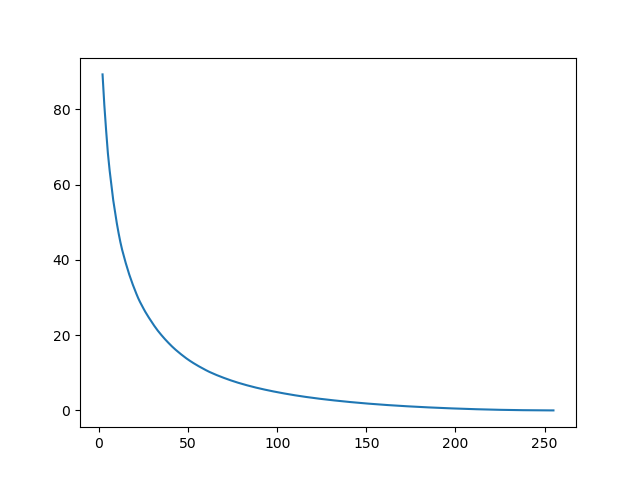
\includegraphics[height=8cm]{./digits_k_variance.png}

Auf dem Plot ist kein echten "Elbogen" zu sehen oder erst bei k=80, wobei das initiale Datensatz
nur 256 Dimensionen hat.

\section*{2D Visualisierung von den einzelnen Cluster bei dem Zifferklassifizierungsproblem}


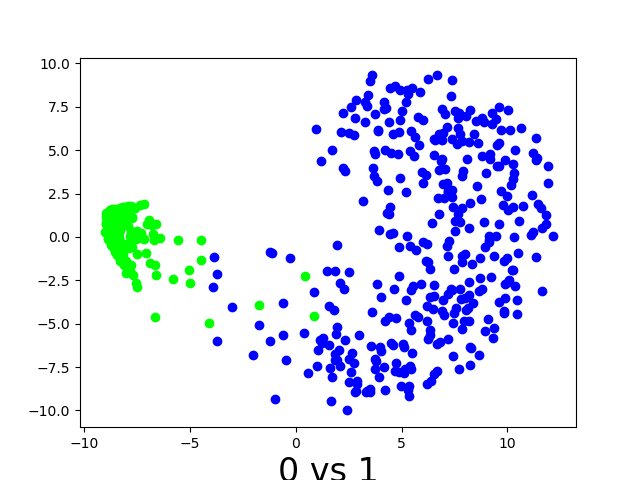
\includegraphics[height=2cm]{./figs/0vs1.png}
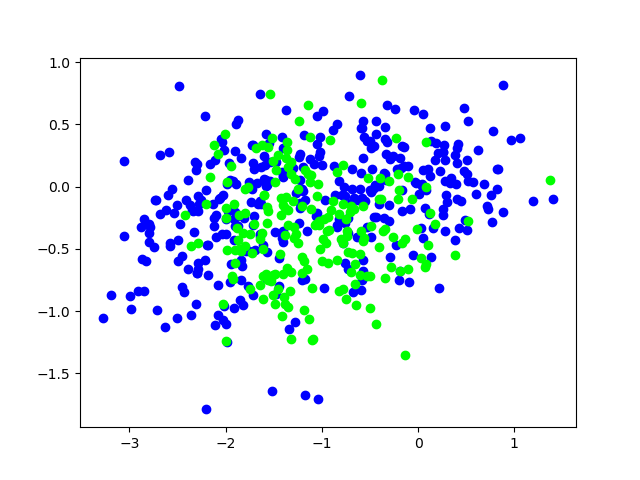
\includegraphics[height=2cm]{./figs/0vs2.png}
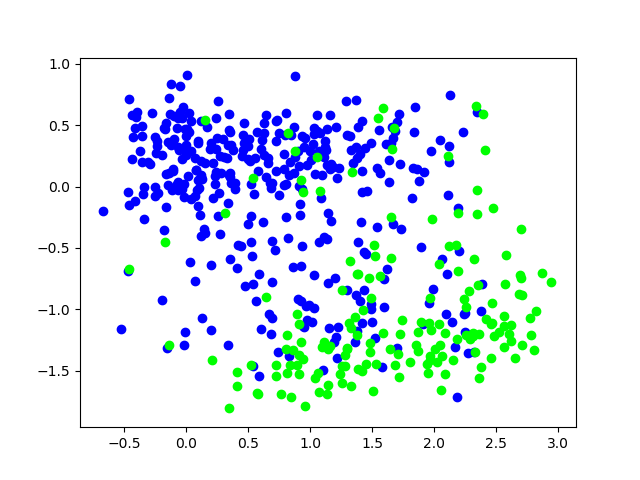
\includegraphics[height=2cm]{./figs/0vs3.png}
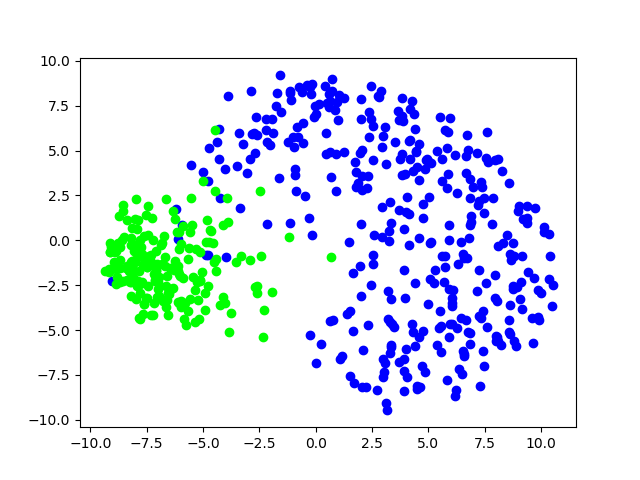
\includegraphics[height=2cm]{./figs/0vs4.png}
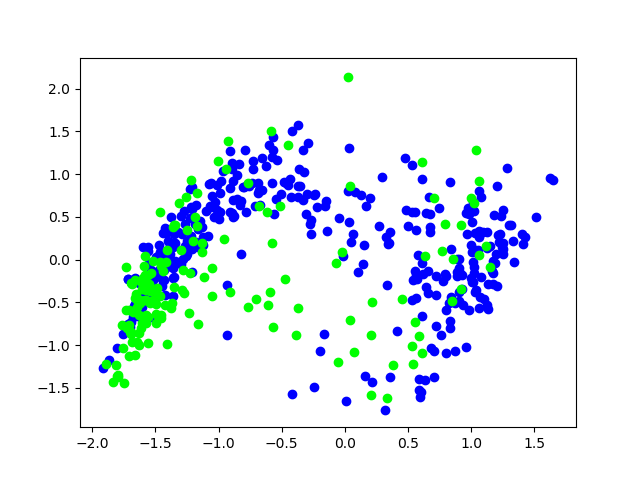
\includegraphics[height=2cm]{./figs/0vs5.png}
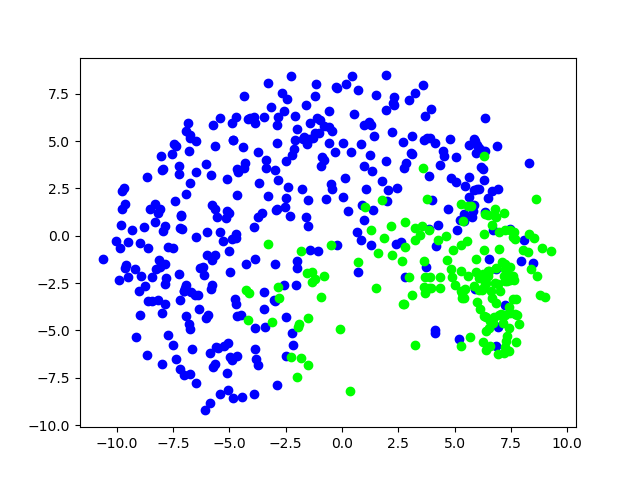
\includegraphics[height=2cm]{./figs/0vs6.png}
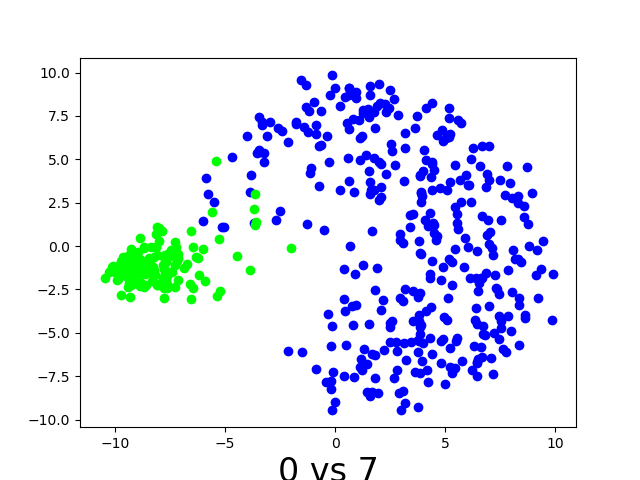
\includegraphics[height=2cm]{./figs/0vs7.png}
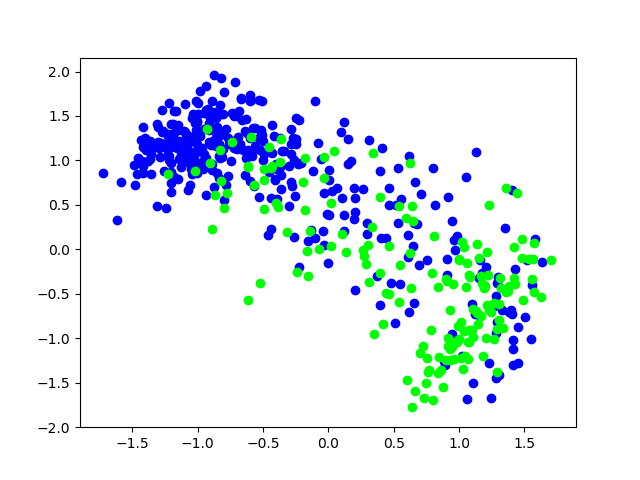
\includegraphics[height=2cm]{./figs/0vs8.png}
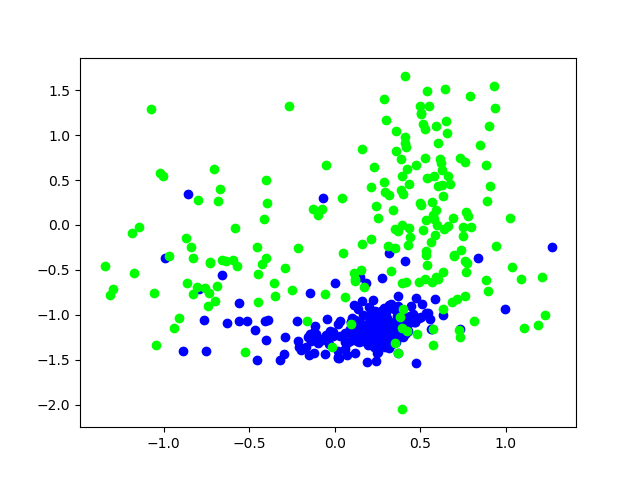
\includegraphics[height=2cm]{./figs/1vs2.png}
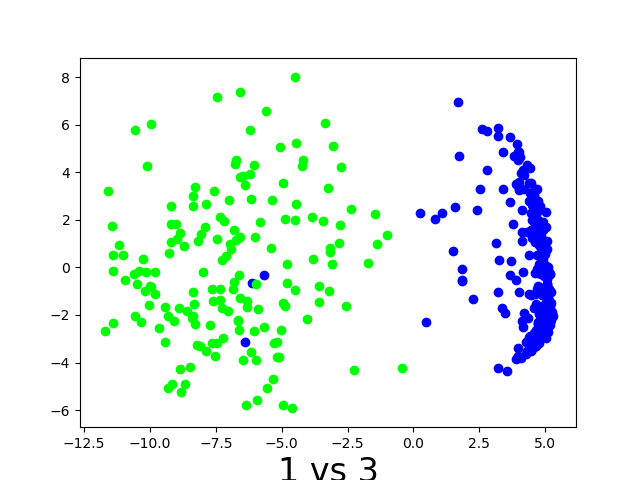
\includegraphics[height=2cm]{./figs/1vs3.png}
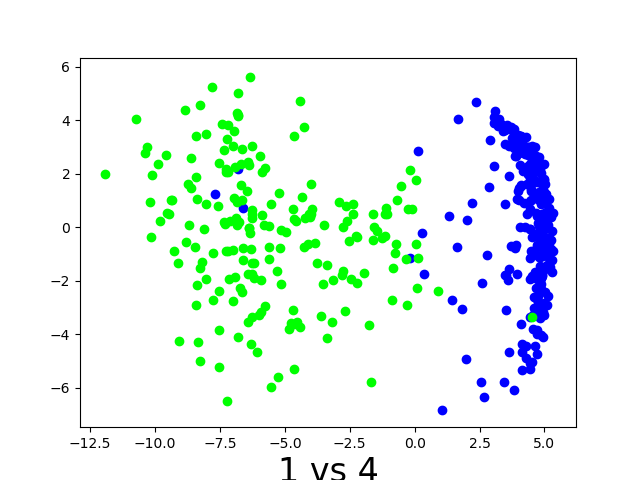
\includegraphics[height=2cm]{./figs/1vs4.png}
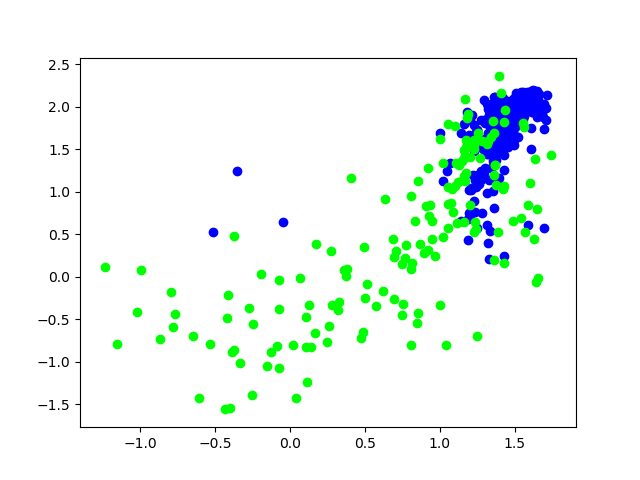
\includegraphics[height=2cm]{./figs/1vs5.png}
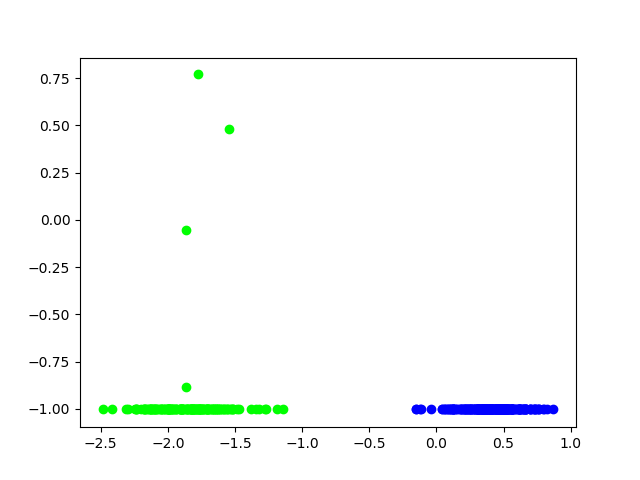
\includegraphics[height=2cm]{./figs/1vs6.png}
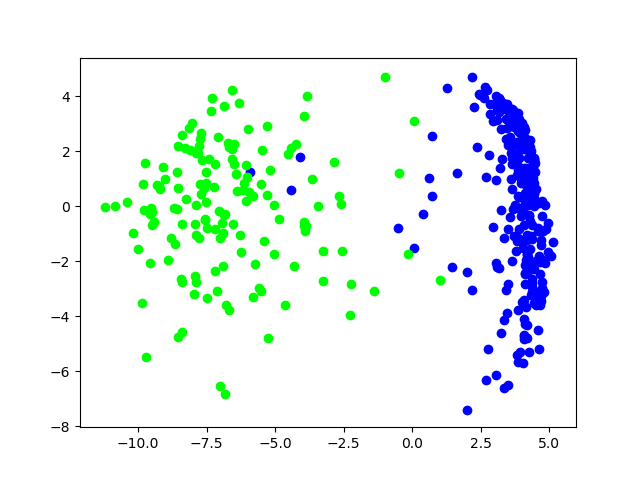
\includegraphics[height=2cm]{./figs/1vs7.png}
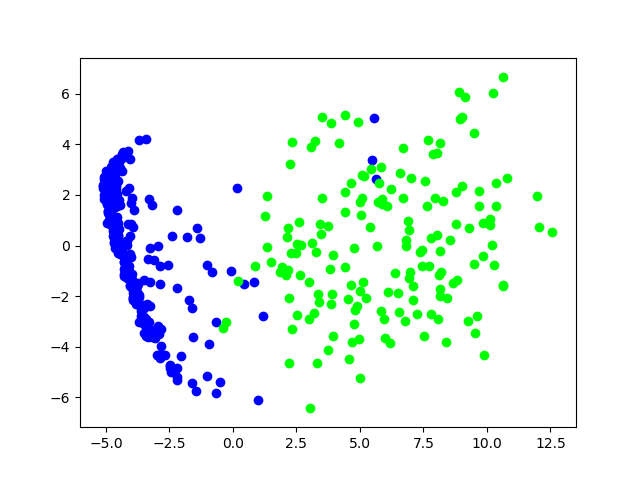
\includegraphics[height=2cm]{./figs/1vs8.png}
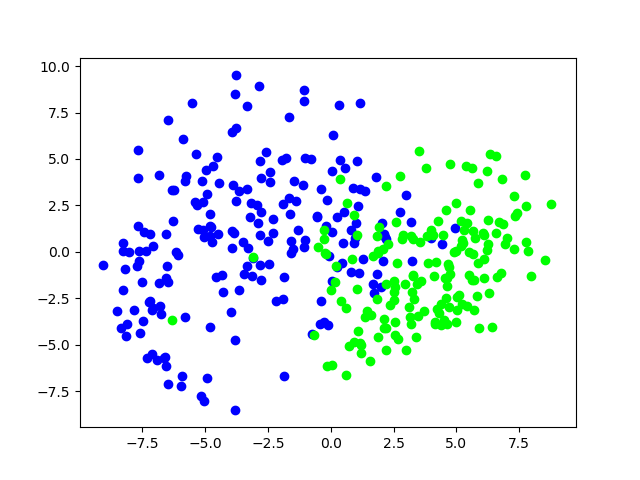
\includegraphics[height=2cm]{./figs/2vs3.png}
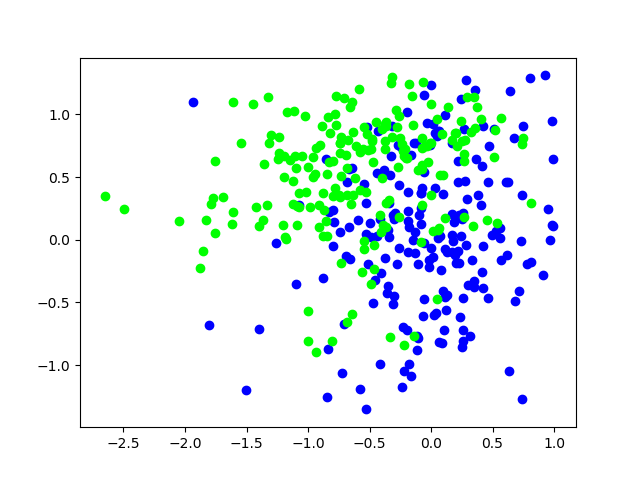
\includegraphics[height=2cm]{./figs/2vs4.png}
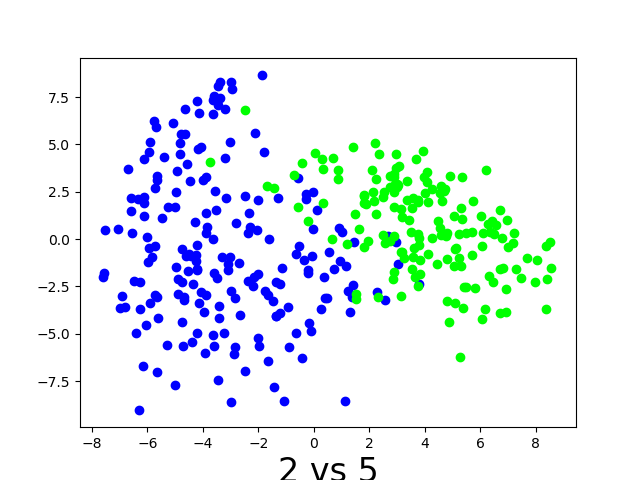
\includegraphics[height=2cm]{./figs/2vs5.png}
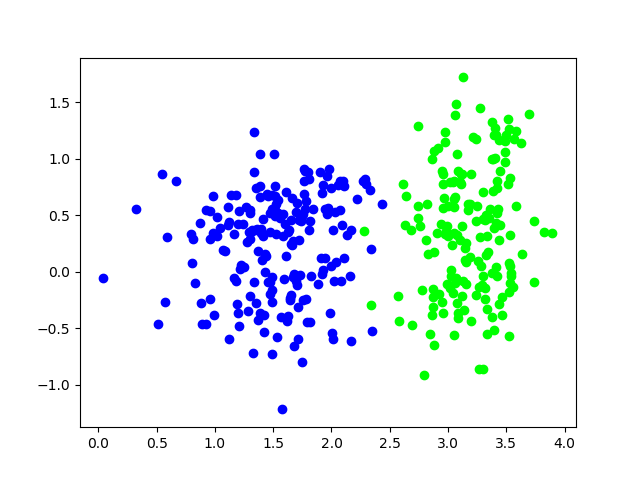
\includegraphics[height=2cm]{./figs/2vs6.png}
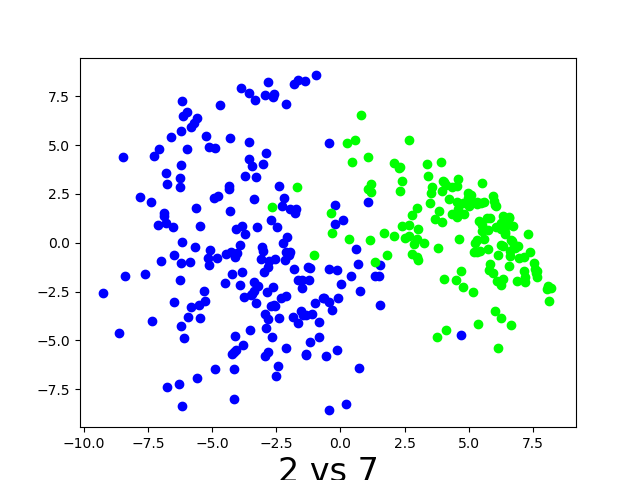
\includegraphics[height=2cm]{./figs/2vs7.png}
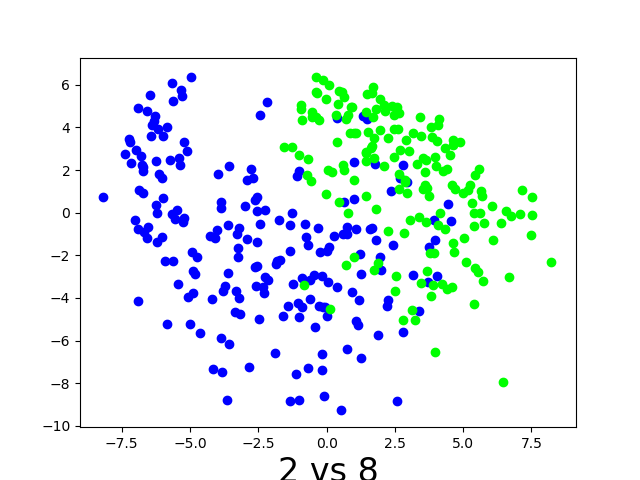
\includegraphics[height=2cm]{./figs/2vs8.png}
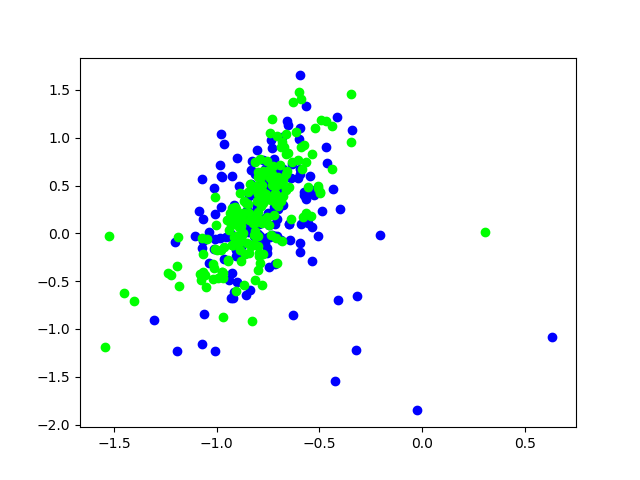
\includegraphics[height=2cm]{./figs/3vs4.png}
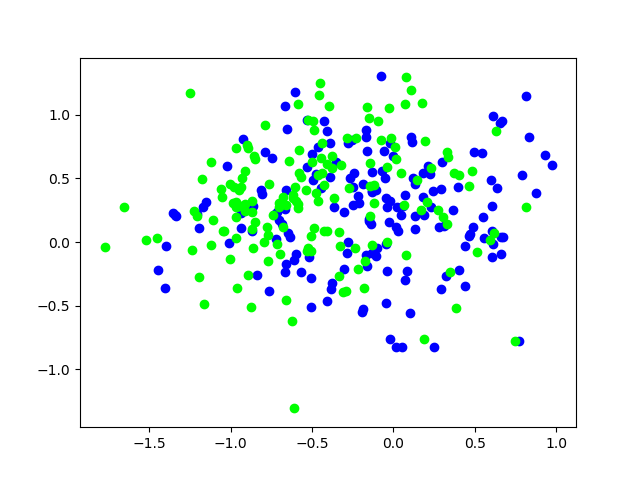
\includegraphics[height=2cm]{./figs/3vs5.png}
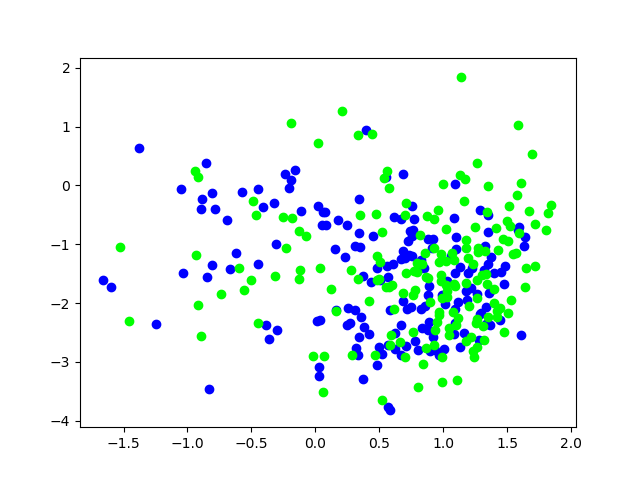
\includegraphics[height=2cm]{./figs/3vs6.png}
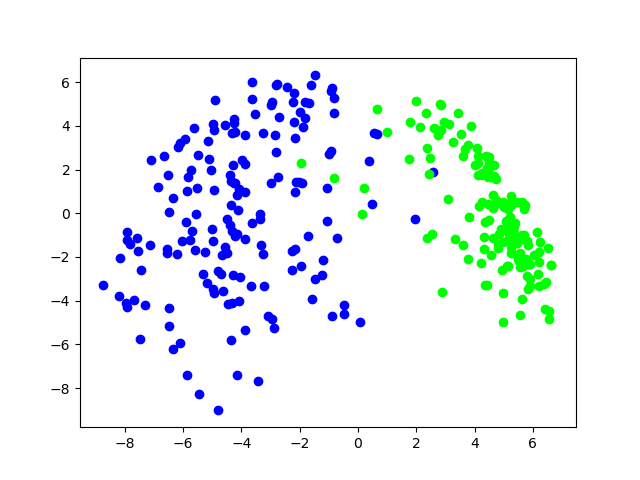
\includegraphics[height=2cm]{./figs/3vs7.png}
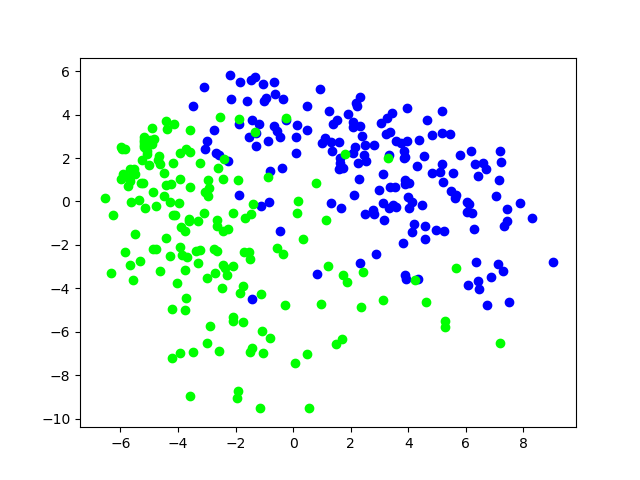
\includegraphics[height=2cm]{./figs/3vs8.png}
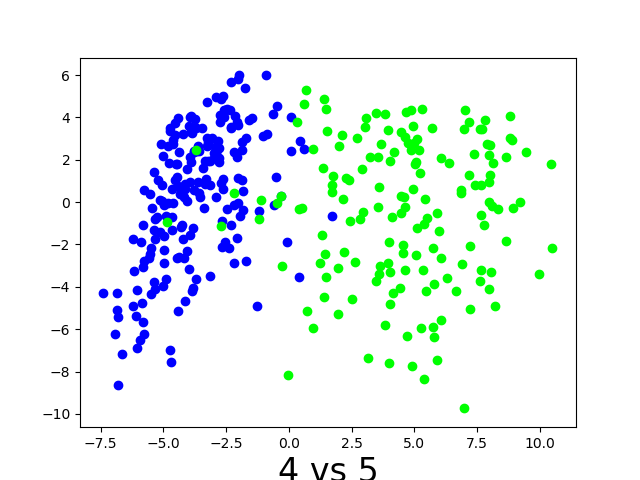
\includegraphics[height=2cm]{./figs/4vs5.png}
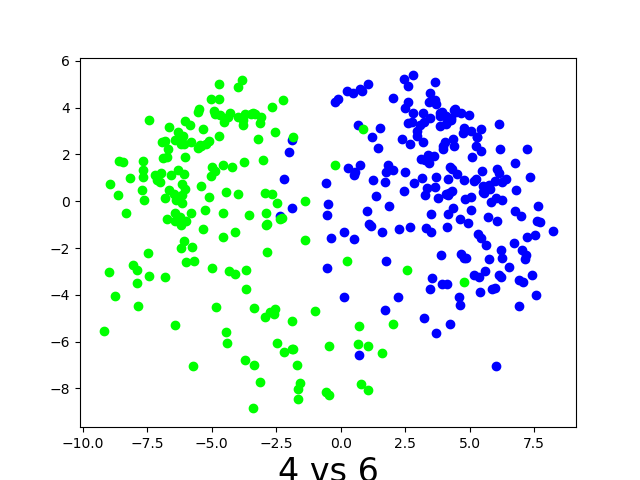
\includegraphics[height=2cm]{./figs/4vs6.png}
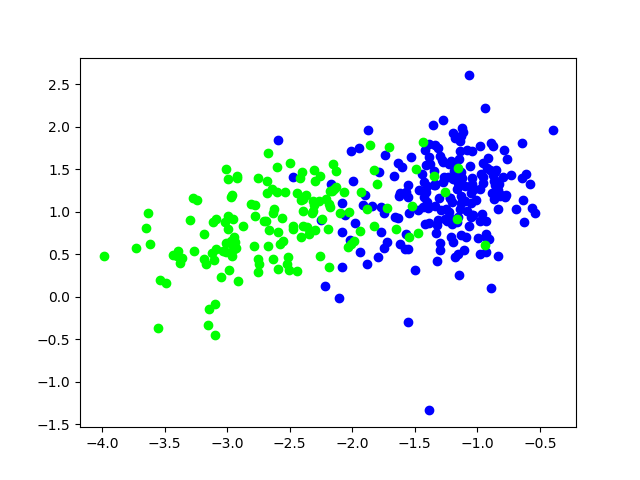
\includegraphics[height=2cm]{./figs/4vs7.png}
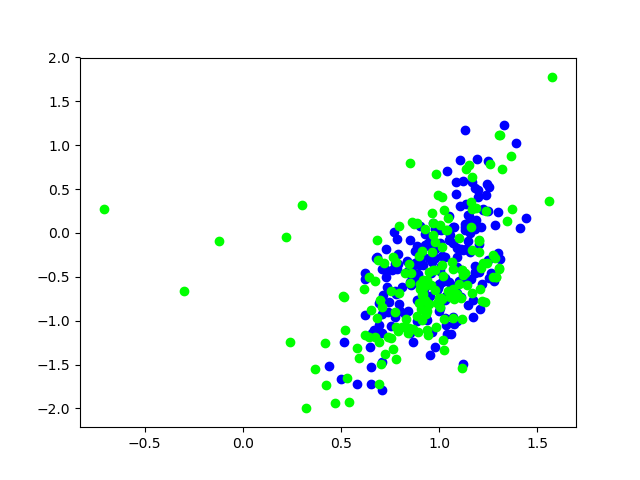
\includegraphics[height=2cm]{./figs/4vs8.png}
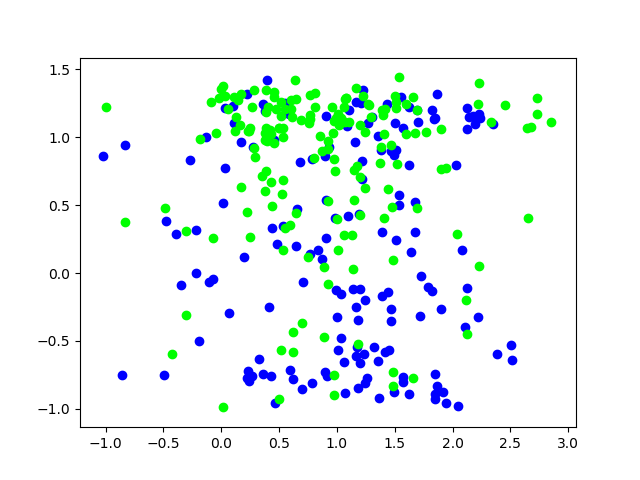
\includegraphics[height=2cm]{./figs/5vs6.png}
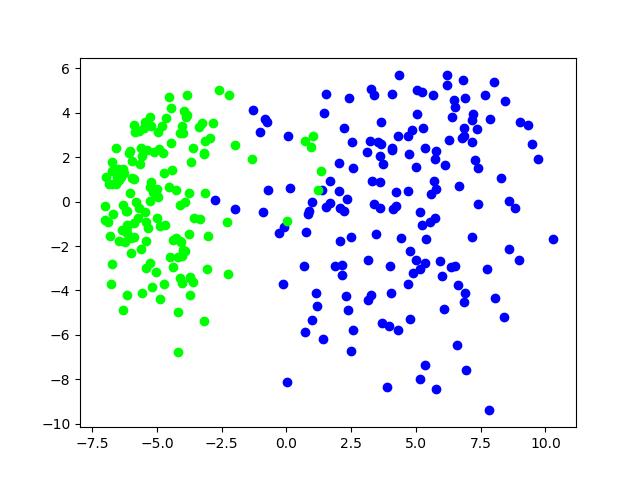
\includegraphics[height=2cm]{./figs/5vs7.png}
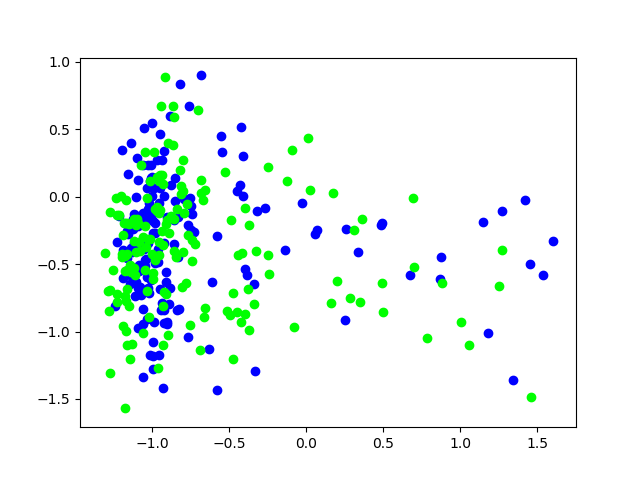
\includegraphics[height=2cm]{./figs/5vs8.png}
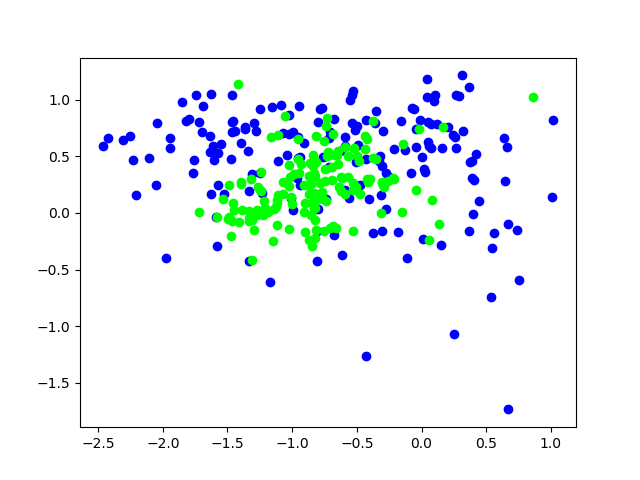
\includegraphics[height=2cm]{./figs/6vs7.png}
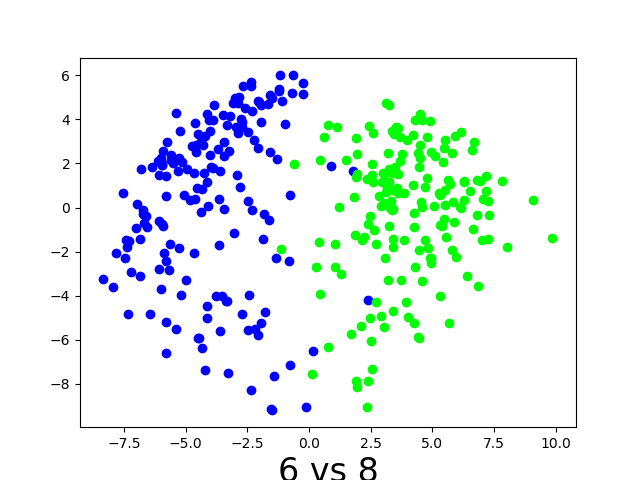
\includegraphics[height=2cm]{./figs/6vs8.png}
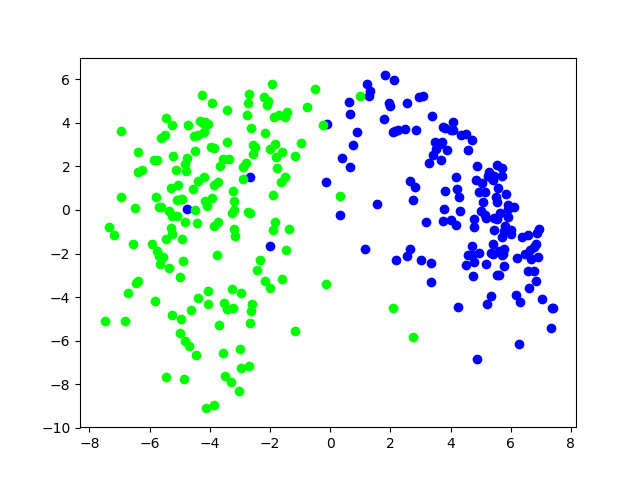
\includegraphics[height=2cm]{./figs/7vs8.png}


Wie man sieht, sind einige Ziffer linear von einander separierbar (z.B. 1 und 3) und andere
gar schwer von einander unterscheidbar (in 2D Raum, 2 und 8). Man sieht, dass es auch einige gibt, die in den meisten
Fällen gut unterscheidbar sind, aber haben auch einige Exemplare, die ganz ähnlich sind (z. B. 3 und 5, wenn man das
obere Teil von je Ziffer nicht gut geschrieben hat ist das untere ja gleich).


Hier wurde aus dem ganzen Datensatz nur das jeweilige Paar genommen und die Dimensionen davon wurden reduziert.
Wenn man aber PCA auf dem ganzen Datensatz anwendet, kriegt man nicht so gute Ergebnisse. Deswegen wurden wir vermuten,
das man mit deutlich bessere Ergebnisse bekommen würde, wenn man ein binäres Klassifikator benutzt und damit zusammen
PCA anwendet.

\section*{Eigenfaces}

Wir haben PCA auf dem Datensatz von menschlichen Gescihten angewandt. Die dabei berechnete Hauptkomponenten
(die Eigenvektoren der Kovarianzmatrix) nennt man "Eigenfaces". Wie man auf dem nächsten Plot sieht, ist
das "Elbogen", also das Punkt, ab dem man nicht viel Varianz mehr gewinnt bei weiteren Hauptkomponenten, erst
bei Circa 320 Dimensionen. Die verlorene Varianz hört aber schon bei circa 30 echt drastisch zu sinken, deswegen
haben wir 30 Hauptkomponenten genommen.

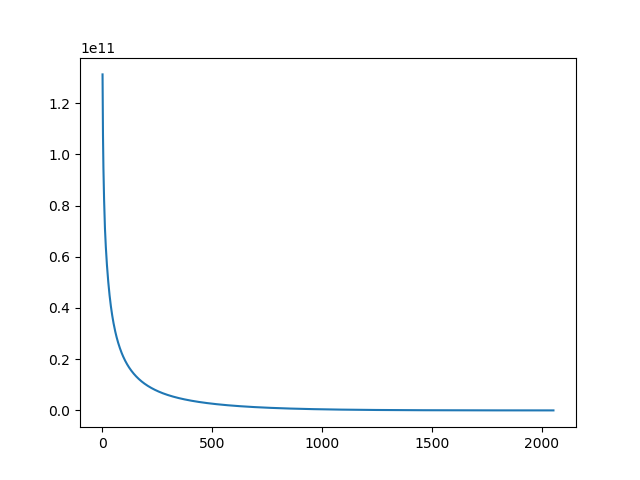
\includegraphics[height=8cm]{./eigenfaces_variance_for_k.png}

\section*{Hauptkomponenten des Gesichtsdatensatzes (a.k.a Eigenfaces)}

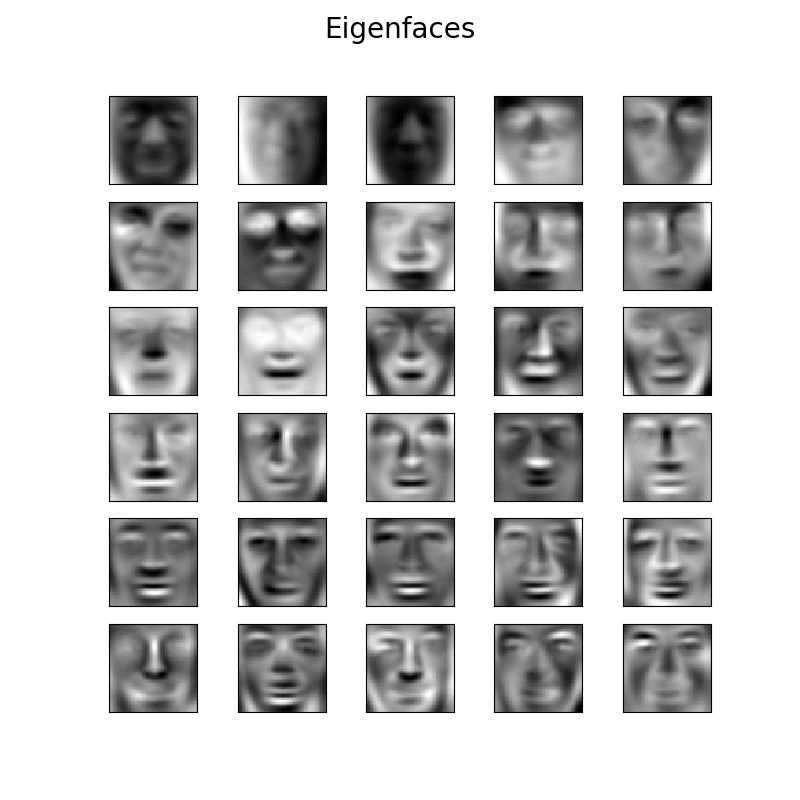
\includegraphics[height=8cm]{./eigenfaces.png}

\section*{Erklärung der PCA Implementierung}

\section*{Fit Methode}

Diese Methode berechnet unsere Hauptkomponenten und damit auch die Transformationsmatritze, mit der man
ein Datensatz von n auf k Dimensionen reduziert. Hier wurde PCA genaus so wie in der Vorlesung auf eine höhe
Abstraktionsebene implementiert, interessanter sind also eigentlich die Hilfsfunktionen.


\begin{lstlisting}[style=py]
    def fit(self, X):
        sorted_k_eig_vectors = PCA.get_sorted_eig_vec(X, self.k)
        self.principal_components = sorted_k_eig_vectors
        self.transformation_matrix = sorted_k_eig_vectors.T
\end{lstlisting}

\section*{Hilfsfunktionen}

Wir berechnen die Kovarianzmatrix mit np.cov. Hier ist wichtig entweder das tronsponierte Datensatz
zu benutzen, oder rowvar auf False zu setzen, damit man die Die Verhältnisse der Features im Datensatz und nicht
der Samples.

Nachher können wir mit Hilfe von np.linalg.eigh die Eigenvektoren und iher entsprechende Eigenwerte berechnen.
Hier ist ganz wichtig, dass die Eigenvektoren die Spalten der zurückgegebener Matrix sind. Das haben wir
initial nicht verstanden und ziemlich viel Zeit deswegen beim Debugging verbracht.

Danach kann man leicht mit argsort() die Indizes bekommen, die die Eigenwerte sortieren und damit die
Eigenvektoren sortieren und zurückgeben. Da die Eigenvektoren die Spalten sind, muss man hier aufpassen.

Die sortierte Eigenwerte brauchen wir für die Berechnung der verlorenen Kovarianz bei k Dimensionen.

\begin{lstlisting}[style=py]
@staticmethod
    def get_eig_values_sort_args(eig_values, k=None):
        if k is None:
            k = len(eig_values)

        # reverse sorted, first k components
        return eig_values.argsort()[::-1][:k]

    @staticmethod
    def get_eig_vec_and_val(X):
        covariance_matrix = np.cov(X, rowvar=False)
        # the covariance matrix is always symmetric, we don't need to bother any further
        # therefore, we can also use eigh instead of eig
        return np.linalg.eigh(covariance_matrix)

    @staticmethod
    def get_sorted_eig_vec(X, k=None):
        eig_values, eig_vectors = PCA.get_eig_vec_and_val(X)
        sort_args = PCA.get_eig_values_sort_args(eig_values, k)

        return eig_vectors[:,sort_args].T

    @staticmethod
    def get_sorted_eig_values(X, k=None):
        eig_values, eig_vectors = PCA.get_eig_vec_and_val(X)
        # assert(np.all(eig_values >= 0))  # yep, all good
        sort_args = PCA.get_eig_values_sort_args(eig_values, k)

        return eig_values[sort_args]
\end{lstlisting}

\section*{Plotting der verlorenen Varianz bei k Dimensionen}

Die Differenz von der Summe aller Eigenwerte mit der Summe von den benutzten (diese, der benutzten Hauptkomponenten) ist
eine gute Möglichkeit zu plotten wie viel von der Varianz verloren wurde bei k Dimension. Ein Idealwert wäre also 0,
wir wollen aber sehen, ab wie viele Dimensionen der Wert deutlich langsamer senkt.

\begin{lstlisting}[style=py]
@staticmethod
    def plot_variance_for_k(X, save_plot_name=None):
        sorted_eig_values = PCA.get_sorted_eig_values(X)
        total_variance = sorted_eig_values.sum()
        ks = np.arange(2, len(X[0]), 1)

        variance_diffs = np.vectorize(lambda k: abs(total_variance - sorted_eig_values[:k].sum()))(ks)
        plt.plot(ks, variance_diffs)

        if save_plot_name is not None:
            plt.savefig(save_plot_name + '.png')
        else:
            plt.show()
\end{lstlisting}

\section*{Transform bzw. Fit-Transform Methoden}

Wie unten erklärt, wenn man je x aus dem Datensatz mit je Hauptkomponente multipliziert
bekommt man x in den reduzierten Raum.

Bsp: xi * (e1, e2, ..., ek) = xi representiert durch die k Hauptkomponenten

Wir speichern bei der Fit-Methode die Transformationsmatritze und nutzen diese bei Transform.
So können wir dan weitere Daten erstmal transformieren, bevor wir Vorhersagen machen.

\begin{lstlisting}[style=py]
    def transform(self, X):
        '''
        (x11 x12 ... x1n )             (e11 e12 ... e1n)T       (x1 projected in subspace)
        (... ... ... ... )      X      (... ... ... ...)    =   (...                     )
        (xm1 xm2 ... xmn )             (ek1 ek2 ... ekn)        (xm projected in subspace)

        self.transformation_matrix is the already transponded matrix where each row is an eigenvector

        :param X: data set, each row represents a sample
        :return: X in the space defined by the first k eigenvectors of the fit data set
        '''

        return X.dot(self.transformation_matrix)

    def fit_transform(self, X):
        self.fit(X)
        return self.transform(X)
\end{lstlisting}

\section*{Vollständiges Code (auch für Plotting, Eigenfaces, Helpers usw.)}

PCA.py
\begin{lstlisting}[style=py]
from Classifier import Classifier
import numpy as np
from matplotlib import pyplot as plt


class PCA(Classifier):
    def __init__(self, k):
        self.transformation_matrix = None
        self.k = k
        self.X_mean = None
        self.principal_components = None

    @staticmethod
    def get_eig_values_sort_args(eig_values, k=None):
        if k is None:
            k = len(eig_values)

        # reverse sorted, first k components
        return eig_values.argsort()[::-1][:k]

    @staticmethod
    def get_eig_vec_and_val(X):
        covariance_matrix = np.cov(X, rowvar=False)
        # the covariance matrix is always symmetric, we don't need to bother any further
        # therefore, we can also use eigh instead of eig
        return np.linalg.eigh(covariance_matrix)

    @staticmethod
    def get_sorted_eig_vec(X, k=None):
        eig_values, eig_vectors = PCA.get_eig_vec_and_val(X)
        sort_args = PCA.get_eig_values_sort_args(eig_values, k)

        return eig_vectors[:,sort_args].T

    @staticmethod
    def get_sorted_eig_values(X, k=None):
        eig_values, eig_vectors = PCA.get_eig_vec_and_val(X)
        # assert(np.all(eig_values >= 0))  # yep, all good
        sort_args = PCA.get_eig_values_sort_args(eig_values, k)

        return eig_values[sort_args]

    def fit(self, X):
        '''
        Finds the largest k eigenvalues and their corresponding eigenvectors from the
        covariance matrix of the dataset and saves the transformation matrix
        which can be used to project a data set from it's original space to
        the space defined by those eigenvectors and their corresponding eigenvalues
        '''

        sorted_k_eig_vectors = PCA.get_sorted_eig_vec(X, self.k)
        self.principal_components = sorted_k_eig_vectors
        self.transformation_matrix = sorted_k_eig_vectors.T

    def transform(self, X):
        '''
        (x11 x12 ... x1n )             (e11 e12 ... e1n)T       (x1 projected in subspace)
        (... ... ... ... )      X      (... ... ... ...)    =   (...                     )
        (xm1 xm2 ... xmn )             (ek1 ek2 ... ekn)        (xm projected in subspace)

        self.transformation_matrix is the already transponded matrix where each row is an eigenvector

        :param X: data set, each row represents a sample
        :return: X in the space defined by the first k eigenvectors of the fit data set
        '''

        return X.dot(self.transformation_matrix)

    def fit_transform(self, X):
        self.fit(X)
        return self.transform(X)

    @staticmethod
    def plot_variance_for_k(X, save_plot_name=None):
        sorted_eig_values = PCA.get_sorted_eig_values(X)
        total_variance = sorted_eig_values.sum()
        ks = np.arange(2, len(X[0]), 1)

        variance_diffs = np.vectorize(lambda k: abs(total_variance - sorted_eig_values[:k].sum()))(ks)

        plt.plot(ks, variance_diffs)

        if save_plot_name is not None:
            plt.savefig(save_plot_name + '.png')
        else:
            plt.show()


\end{lstlisting}

Helpers.py
\begin{lstlisting}[style=py]
import numpy as np
import math
import os
from matplotlib import pyplot as plt


def plot_multiple_images(title, images, data_set_dimensions, cols=5, fig_name=None):
    rows = math.ceil(len(images) / cols)
    plt.figure(figsize=(8,8))
    plt.suptitle(title, size=20)

    for i, component in enumerate(images):
        plt.subplot(rows, cols, i + 1)
        component += abs(component.min())
        component *= (1.0 / component.max())
        image = np.reshape(component, (data_set_dimensions, data_set_dimensions))
        plt.imshow(image, cmap=plt.cm.binary)
        plt.xticks(())
        plt.yticks(())

    if fig_name is not None:
        file_name = os.path.join(os.path.dirname(__file__), './{}'.format(fig_name))
        plt.savefig(file_name)
    else:
        plt.show()
\end{lstlisting}

Parser.py
\begin{lstlisting}[style=py]
import csv
import numpy as np
import pandas as pd
import os
from sklearn.model_selection import train_test_split


def parse_data(file_name, sep=' '):
    file_name = os.path.join(os.path.dirname(__file__), './Dataset/{}'.format(file_name))
    return pd.read_csv(file_name, header=None, na_filter=True, sep=sep).as_matrix()


def get_points_and_labels_from_data(data, label_idx=0):
    points = (np.array(data[:, 1:], dtype=np.float64) if label_idx == 0 else
              np.array(data[:, :label_idx], dtype=np.float64))
    labels = np.array(data[:,label_idx])

    return points, labels


def get_data_set(file_name, sep=' ', label_idx=0, seed=4):
    data = parse_data(file_name, sep)
    X, y = get_points_and_labels_from_data(data, label_idx)
    # for determined results we use a seed for random_state, so that data is always split
    X_train, X_test, y_train, y_test = train_test_split(X, y, train_size=0.7, test_size=0.3,
                                                        random_state=seed)

    return X_train, X_test, y_train, y_test


def extract_classes_from_data_set(X, y, classes):
    labels_are_numbers = False

    try:
        a = int(y[0])
        labels_are_numbers = True
    except:
        pass

    is_from_classes = np.vectorize(lambda y: (int(y) if labels_are_numbers else y) in classes)
    filter_arr = is_from_classes(y)
    return X[filter_arr], y[filter_arr]

\end{lstlisting}

digits\_classification.py
\begin{lstlisting}[style=py]
import numpy as np
from sklearn.discriminant_analysis import LinearDiscriminantAnalysis as LDA
from PCA import PCA
from Parser import get_data_set

X_train, X_test, y_train, y_test = get_data_set('digits.data')

pca_230 = PCA(230)
train_transformed_230 = pca_230.fit_transform(X_train)
test_transformed_230 = pca_230.transform(X_test)

pca_30 = PCA(30)
train_transformed_30 = pca_30.fit_transform(X_train)
test_transformed_30 = pca_30.transform(X_test)

PCA.plot_variance_for_k(X_train)

prediction_non_transformed = LDA().fit(X_train, y_train).predict(X_test)
score_non_transformed = np.mean(prediction_non_transformed == y_test)
print('Score LDA without PCA: {}'.format(score_non_transformed))

prediction_transformed_230 = LDA().fit(train_transformed_230, y_train).predict(test_transformed_230)
score_transformed_230 = np.mean(prediction_transformed_230 == y_test)
print('Score LDA with PCA, k={}: {}'.format(230, score_transformed_230))

prediction_transformed_30 = LDA().fit(train_transformed_30, y_train).predict(test_transformed_30)
score_transformed_30 = np.mean(prediction_transformed_30 == y_test)
print('Score LDA with PCA, k={}: {}'.format(30, score_transformed_30))

\end{lstlisting}

demo\_digits\_PCA.py
\begin{lstlisting}[style=py]
from matplotlib import pyplot as plt
import numpy as np
from sklearn.decomposition import PCA as PCA_sklearn
from PCA import PCA
from Parser import parse_data, get_points_and_labels_from_data, extract_classes_from_data_set

data = parse_data('digits_test.data')
X, y = get_points_and_labels_from_data(data)

for a in range(10):
    for b in range(a+1, 10, 1):
        X_extracted, y_extracted = extract_classes_from_data_set(X, y, [a,b])
        X_transformed = PCA(2).fit_transform(X_extracted)
        X_a_idx = y_extracted.astype(int) == a
        X_a = X_transformed[X_a_idx]
        X_b = X_transformed[np.invert(X_a_idx)]

        plt.scatter(X_a[:,0], X_a[:,1], c='#0000FF')
        plt.scatter(X_b[:,0], X_b[:,1], c='#00FF00')
        plt.xlabel('{} vs {}'.format(a, b), fontsize=24)
        plt.savefig('figs/{}vs{}.png'.format(a,b))
        plt.clf()

\end{lstlisting}

eigenfaces.py
\begin{lstlisting}[style=py]
from PCA import PCA
from Helpers import plot_multiple_images
import numpy as np
import math
import glob
import os
import cv2


def read_pgm(file_name):
    return cv2.imread(file_name, -1)

data_folder = os.path.abspath(os.path.join(os.path.dirname(__file__), './Dataset'))
files = glob.glob(data_folder + '/lfwcrop_grey/faces/*.pgm')
data_set = []

for file in files:
    image = read_pgm(file)
    data_set.append(image.flatten())

data_set = np.array(data_set)

# drops quickly until about k=320
# but really quickly until about 30, plus we can't really submit 320 eigenfaces for this homework...
# PCA.plot_variance_for_k(data_set, save_plot_name='eigenfaces_variance_for_k')


pca_eigenfaces = PCA(30)
pca_eigenfaces.fit(data_set)
data_set_dimensions = int(math.sqrt(len(data_set[0])))
principal_components = pca_eigenfaces.principal_components

plot_multiple_images('Eigenfaces', principal_components, data_set_dimensions, fig_name='eigenfaces.png')

\end{lstlisting}


% /////////////////////// END DOKUMENT /////////////////////////
\end{document}
